\subsection{Smart Locks}
\label{sec:sota_smart_locks}
	Da sich Architektur und Funktionsmechanismen in manchen Punkten je nach Hersteller unterscheiden, gelten die im Folgenden dargelegten technischen Erklärungen, soweit nicht explizit erwähnt, für das Smart Lock von der Firma August. 
    \medskip\\
    \noindent Smart Locks sind ,,elekromechanische Türschlösser``, die sich dadurch auszeichnen, dass sie für einen Nutzer mit einer Smartphone-App steuerbar sind und mittels eines kabellosen Standards wie Bluetooth (siehe \fref{sec:sota_iot_protocols}) für kurze Distanzen kommunizieren.
	Als ,,Smart Lock`` werden keine Schlösser bezeichnet, bei denen ein physisches Schloss
	\footnote{beispielweise ein Stiftschloss, welches mit einem herkömmlichen Schlüssel geöffnet werden kann} 
	mit einem Ziffernblock ersetzt wurde oder sich nicht mit anderen Geräten innerhalb des \gls{iot} in irgendeiner Weise verbinden.\cite{Ho2016}
	
	\subsubsection{Typische Architekturen und Gemeinsamkeiten}
	    In den den doch sehr unterschiedlichen Produkten, die momentan auf dem freien Markt verfügbar sind oder bisher verfügbar waren, lassen sich trotz alledem einige Gemeinsamkeiten erkennen\cite{Ye2017,Fuller2017}. 
    	\noindent Generell besteht ein Smart Lock-System aus folgenden Bestandteilen (vgl. \fref{fig:sl_arch}):
    	\begin{enumerate}[noitemsep]
    		\item einem elektrischen Schloss oder einer elektronischen Erweiterung eines vorhandenen Schlosses
    		\item mindestens einem Nutzer, welcher durch sein Endgerät, meist ein Smartphone, identifiziert wird
    		\item einem herstellereigenen Server
    		\item einem Webinterface
    		\item optional einem Zubehörgerät, welches erlaubt dem Schloss mit dem Internet zu kommunizieren
    	\end{enumerate}
    
    	\begin{figure}[H]
    		\centering
    		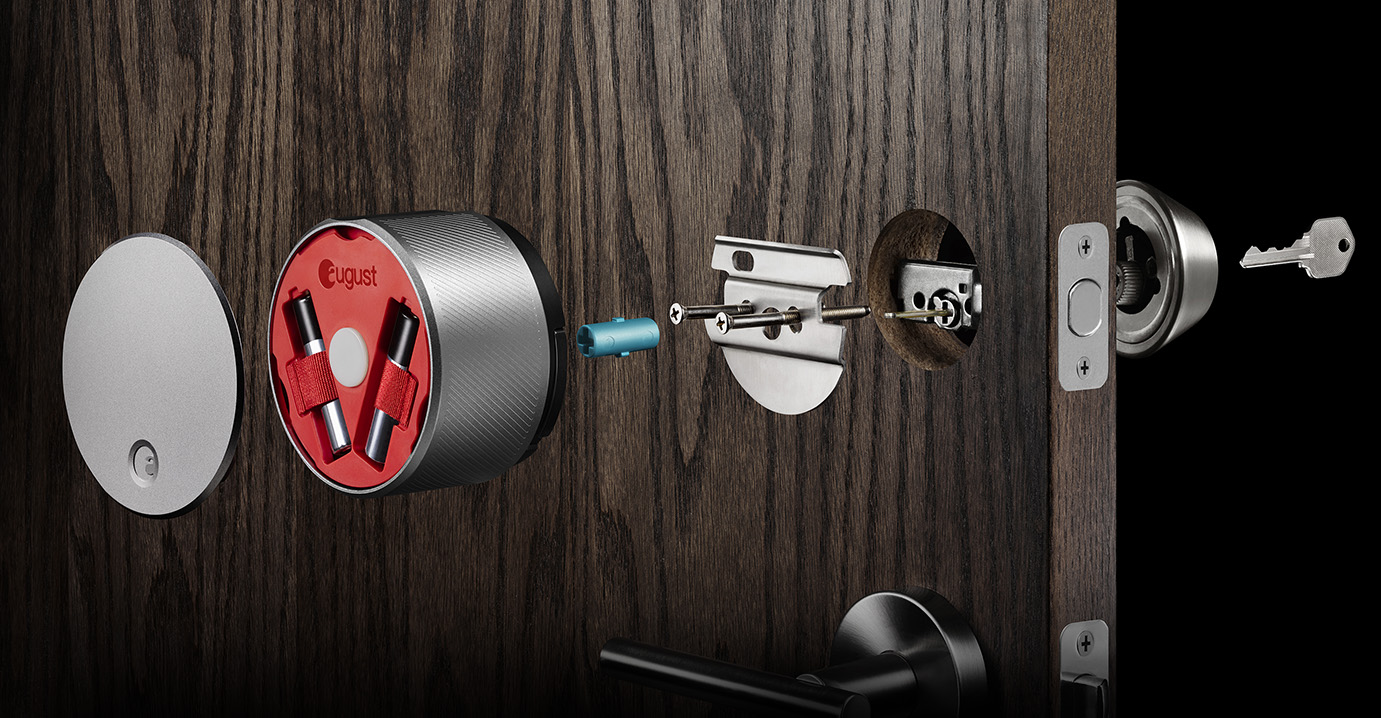
\includegraphics[width=0.9\textwidth]{graphics/august_2.jpg}
    		\caption{Bestandteile eines August Smart Lock Pro\cite{August}}
    		\label{fig:august1}
    	\end{figure}
    
	    \noindent Das Schloss selbst ist an der Außen- und/oder Innenseite einer Tür angebracht (vgl. \fref{fig:august1}) und erweitert ein vorhandenes Schloss elektronisch oder ist selbst in Form eines Vorhängeschlosses\cite{Ho2016}. 
		Zum System gehört in den meisten Fällen eine mobile Applikation für ein Smartphone zum Öffnen und Schließen des Schlosses, sowie zur Administration\cite{Fuller2017}. 
        Eher seltener beinhaltet das Produkt auch eine Weboberfläche, welche ebenfalls für administrative Aufgaben genutzt werden kann\cite{Ho2016}. 
		Es existiert ein herstellereigener (Remote-)Server, auf dem sich eine authoritative Liste aller Nutzer, sowie deren Rechte befindet. 
        Diese bildet die Grundlage zur Realisierung der Zugriffskontrolle.\cite{Fuller2017} 
        Das Öffnen und Schließen erfolgt primär elektronisch mittels eines Buttons per App.
        Alternativ lässt sich das Schloss entweder mit einem sogenannten ,,Keyfob`` 
        \footnote{ein Schlüsselanhänger, auf dem sich ein digitaler Schlüssel befindet} 
        oder einem physischen Schüssel öffnen\cite{Ho2016}. 
        Einige Modelle bieten auch eine Funktion, die die Tür automatisch öffnet sobald sich das Smartphone des Nutzers innerhalb eines bestimmten Radius befindet. 
        Sobald folgende Bedingungen gegeben sind, öffenet sich das Schloss automatisch:
        \begin{itemize}[noitemsep]
        	\item automatisches Öffnen wurde vom Nutzer aktiviert
        	\item der Nutzer hat einen Ort bzw. für Geofencing festgelegt (Bei Geofencing wird mittels \gls{gps} ein Ort festgelegt, um den ein virtueller Zaun gelegt wird. Verlässt oder betritt der Nutzer den festgelegten Radius um den Ort, wird ein Trigger ausgelöst, dem beliebige Aktionen folgen können.)
        	\item der Nutzer befindet sich in Reichweite, um über sein Smartphone mit dem Schloss kommunizieren zu können
        	\item der Nutzer ist berechtigt das Schloss zu öffnen
        \end{itemize}
    	Verlässt der Nutzer den Radius des Geofencings wieder, wird das Schloss automatisch verriegelt.
		Ein optionales Zubehörgerät fungiert als Relay
		\footnote{leitet Nachrichten von mehreren Entitäten in einem Netzwerk (unverändert) weiter}
		, welches sich per \gls{ble} mit dem Schloss verbindet und über das W-LAN Heimnetzwerk des Nutzers mit dem Internet verbindet.
		
    \subsubsection{Typische Funktionen}
		Um das Schloss zu kontrollieren installiert der Nutzer initial eine herstellerspezifische App auf seinem Smartphone und erstellt ein Nutzerkonto auf dem Server des Herstellers. 
		Danach pairt der Nutzer via \gls{ble} sein Gerät mit dem Schloss.\cite{Ho2016} 
		Die Identifikation der verschiedenen Nutzer für administrative Zwecke erfolgt entweder mittels E-Mailadresse oder Telefonnummer. 
		Aus technischer Sicht werden Nutzer anhand eines einzigartiger Schlüssel identifiziert, die der Besitzer des Schlosses nicht kennt.\cite{Fuller2017}\todo[color=orange]{nachlesen} 
		Die Smart Locks enthalten eine eingebaute Funktion, um Zugriffe zu protokollieren. 
		Dazu gehören Aktionen wie \cite{Fuller2017}:
		\begin{itemize}[noitemsep]
			\item von welchem Nutzer eine Funktion genutzt wurde, 
			\item der Zeitpunkt, an dem das Schloss elektronisch geöffnet oder geschlossen wurde,
			\item der Zeitpunkt, an dem das Schloss manuell geöffnet oder geschlossen wurde
			\item wann, wem und von wem Zugriff gewährt oder entzogen wurde
		\end{itemize}
		Die Logs werden asynchron mit der Smartphone App aktualisiert, sobald sich das Gerät des Nutzers in Reichweite des \gls{ble} befindet\citeauthor{Ho2016}.
	
	\subsubsection{Kommunikation}
	    \begin{figure}[H]
    		\centering
    		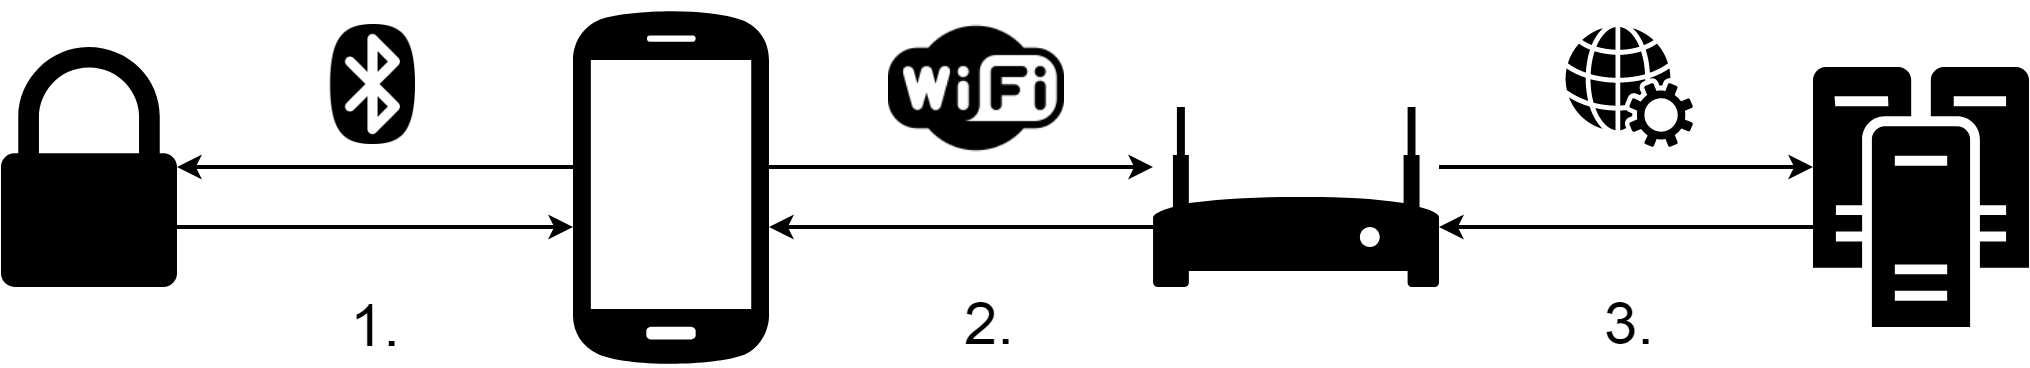
\includegraphics[width=0.9\textwidth]{graphics/gateway_arch.png}
    		\caption{Typische Architektur, welche das Smartphone des Nutzers als Gateway/Proxy nutzt\cite{Ho2016}.}
    		\label{fig:gateway_arch}
    	\end{figure}

        nach \citeauthor{Ho2016}:
        In \fref{fig:sl_arch} abgebildet: Smart Lock hat keine Internetverbindung. 
        Endgerät des Nutzers übernimmt die Funktion eines Proxy/Gateway, welches Informationen zwischen dem Smart Lock und den Servern des Herstellers überträgt. 
        Dies setzt voraus, dass sich das Endgerät in Kommunikationsreichweite für das jeweilige Protokoll (bspw. \gls{ble}) befindet. 
        Direkte Internetverbindung des Smart Locks zur Kommunikation mit dem Server des Herstellers mittels eingebautem Wifi-Modem, welches sich mit dem Netzwerk des Nutzers verbindet. 
        Die Informationen über Rechtevergaben und Gerätezustand etc. werden hier allerdings über das Internet und nicht über lokale Kommunikation (wie \gls{ble}) übertragen. 
        \gls{ble} zwischen Smartphone und Smart Lock wird verwendet für: 
        \begin{itemize}
            \item Athentifizierung des Smartphones des Nutzers 
            \item Nachrichten mit Informationen über gewährten und entzogenen Nutzerrechten
            \item die Smartphone-App bzw. die Logs über Aktivitäten (lock/unlock) informieren
        \end{itemize}

    \subsubsection{Sichereit}
        \paragraph{Rollen und Rechteverteilungen:}
        Relevant: \cite{Ye2017}\cite{Ho2016}
		\subparagraph{Rollen:} Owner(Grant, Revoke, Lock/Unlock, Admin Features wie Zugriffshistorie Lediglich der Nutzer mit der Rolle des Owners kann diese Protokolle einsehen. ), Resident(Lock/Unlock), wiederkehrender Gast (nur Lock/Unlock zu bestimmten Zeitfenstern), temporärer Gast(Lock/Unlock für eine bestimmte Zeit wie 24 Stunden) 
		Die Rolle des Owners wird jenem Gerät vergeben, das sich nach Installation des Smart Locks als erstes mittels \gls{ble} (oder bei einigen Modellen über W-LAN) verbindet. 
   		Die Owner-Rolle kann auf diesem Wege nur einmal vergeben werden. 
   		Bei Wechsel des Besitzers muss das Smart Lock zurückgesetzt werden. 
   		Rollen wieder zu entfernen und somit anderen Nutzers wieder die Rechte zu entziehen, muss Owner sein. 
   		Um die Rechte eines Owners bei einem verlorenen oder gestohlenen zu entziehen, wird entweder eine "Lost Phone"-Funktion angeboten oder ein anderer Nutzer mit der Rolle des Owners entzieht dem nicht mehr vorhandenen Gerät die Rolle. 
   		Der Owner kann das Schloss auch ohne Internetverbindung öffnen/schließen. 
   		Gäste hingegen müssen sich vor der Kommunikation mit dem Schloss gegenüber der dem Server des Herstellers autorisieren lassen. 
		\subparagraph{Rechte:} Lock/Unlock, Lock Activity, Guest List, User Invitation (new Users), User Level Control (update User Role), User Permission Control (e.g. set time slots for guests, revoke permissions from users), Schloss kalibrieren und zurücksetzen\cite{Fuller2017}, Activiy Protokoll ansehen\cite{Fuller2017}, Autolocking/-unlocking akivieren/deaktivieren, eigenen Account löschen
		
		\paragraph{Secret Keys}
		\begin{figure}[H]
			\centering
			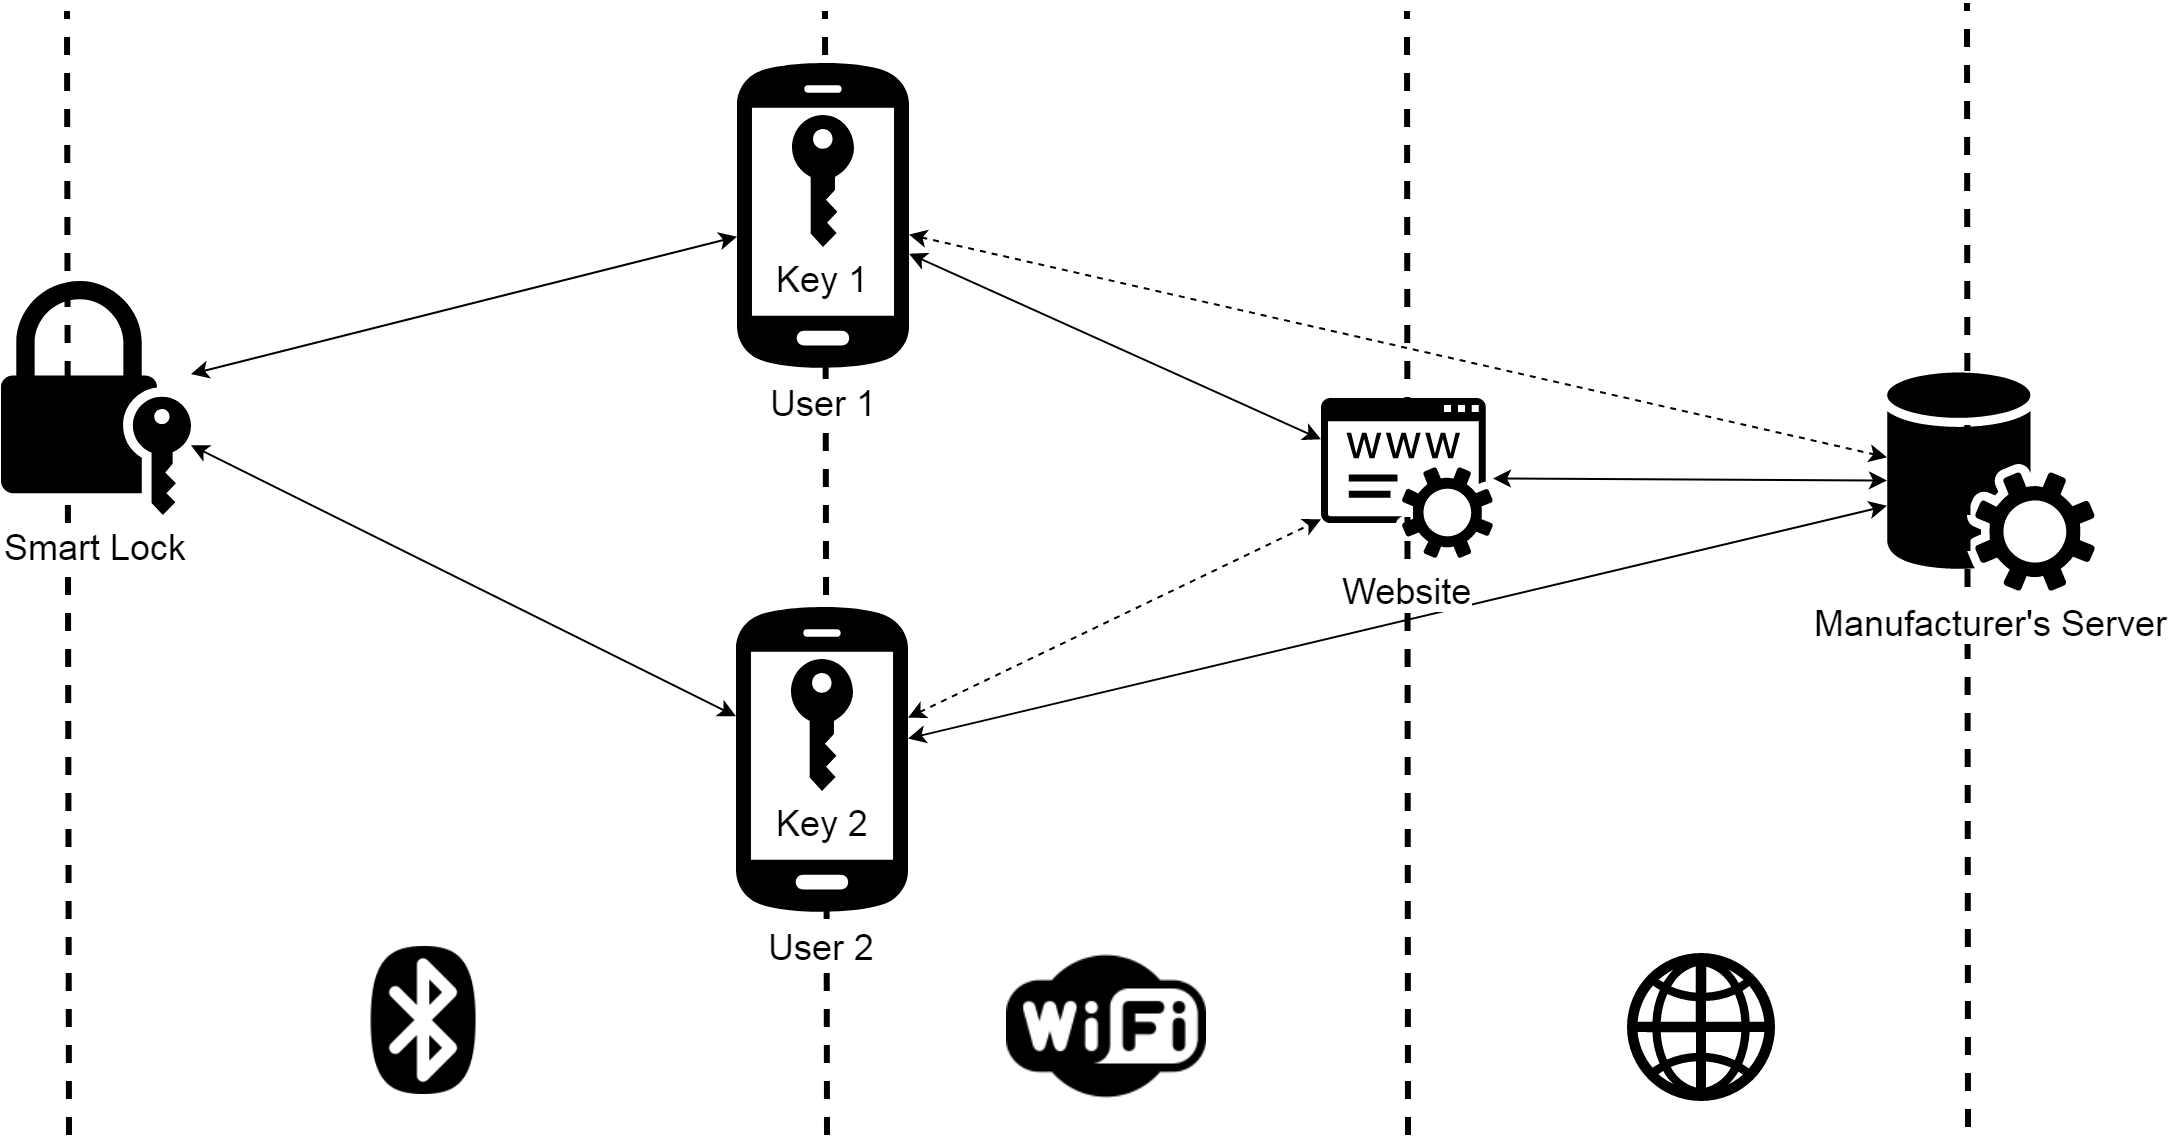
\includegraphics[width=\textwidth]{graphics/sl_arch.png}
			\caption{Beispiel eines Smart Lock-Systems}
			\label{fig:sl_arch}
		\end{figure}
		über Secret Keys\cite{Fuller2017}
		\begin{itemize}
		    \item jede Bluetooth-Verbindungssession bekommmt einen eigenen einzigartigen Session-Key (weiter SK genannt), welcher für Owner wie folgt entsteht:
		    \missingfigure{Wie der Session Key für Owner entsteht}
		        \begin{enumerate}
		            \item Das Smartphone sendet zufällige 64 Bit an das Schloss, welche mit dem offline Keys des Smartphones verschlüsselt werden, an das Schloss
		            \item Das Schloss sendet 64 zufällige Bits, die mit dem offline Key des Smartphones verschlüsselt sind, an das Smartphone zurück
		            \item Das Schloss und das Smartphone entschlüsseln die jeweils erhaltene Nachricht und konkatinieren beide Nachrichten zu einer neuen 128-Bit langen Folge, die im weiteren Verlauf als AES-Key zur Verschlüsselung der Session genutzt wird.
		        \end{enumerate}
		        Gäste, welche keinen "offline Key" zugewiesen bekommen, kommunizieren mit dem Webserver:
		        \missingfigure{Wie der Session Key für Gäste entsteht}
		        \begin{enumerate}
		            \item Das Smartphone des Gasts sendet 64 zufällige Bits als Klartext an den Server
		            \item Der Server verschlüsselt diese 64 Bits mit dem Firmware Key und sendet die verschlüsselten Bits als Nachricht an den Gast zurück
		            \item Der Gast leitet den Ciphertext, welcher von dem Server empfangen wurde, an das Schloss weiter.
		            \item Das Schloss sendet 64 Bits mit XY  verschlüsselt an den Gast, welcher diesen Ciphertext an den Server weiterleitet.
		            \item Der Server entschlüsselt die Nachricht und sendet sie als Klartext per SSL an den Gast.
		            \item Das Schloss und der Gast konkatenieren beide 64-Bit langen Folgen zu einem 128-Bit Schlüssel, welcher als Session Key verwendet wird.
		        \end{enumerate}
		    \item SK wird genutzt, um Nachrichten zwischen dem Schloss und dem Smartphone des Nutzers mit AES zu ver- und entschlüsseln
		    \item Voraussetzung: für das Protokoll, welches den Session Key erstellt müssen bereits im Voraus das Schloss und entweder die Webserver des Herstellers oder das Smartphone des Nutzers einen Secret Key teilen.
		    \item in August können insgesamt 256 Schlüssel (von 0-255 nummeriert) gespeichert werden, wobei Nummer 0 besondere Privilegien hat und als "firmware key" angesehen wird (\textrightarrow Hardcoded und somit anfällig, sollte in falsche Hände geraten).
		        Die Webserver des Herstellers, Nutzer mit der Rolle OWNER und das Schloss selbst kennen den Schlüssel.
		        anderen Keys sind "offline Keys", die zur Initialisierung einer Bluetooth-Session verwendet werden, sollte der Nutzer nicht mit dem Internet verbunden sein
		\end{itemize}
		
		
